\documentclass[11pt,a4paper]{article}

% ---------- Packages ----------
\usepackage[margin=2.7cm]{geometry}
\usepackage[T1]{fontenc}
\usepackage{lmodern}
\usepackage{microtype}
\usepackage{amsmath,amssymb,amsfonts}
\usepackage{booktabs}
\usepackage{tabularx}
\usepackage{enumitem}
\usepackage{xcolor}
\usepackage{hyperref}
\usepackage{graphicx}
\usepackage{tikz}
\usetikzlibrary{arrows.meta,positioning,fit,calc,shadows.blur,decorations.pathmorphing}
\usepackage{pgfplots}
\pgfplotsset{compat=1.18}

\hypersetup{
  colorlinks=true,
  linkcolor=black,
  citecolor=black,
  urlcolor=blue
}

% ---------- Title ----------
\title{\textbf{Existence First: A Universal, Agent-Neutral Theory of Corrigible Persistence}\\
\large An EbE-aligned framework for politics, economics, culture, and AI}
\author{Albert Jan van Hoek}
\date{\today}

% ---------- Helpers ----------
\newcommand{\defterm}[1]{\textbf{#1}}
\newcommand{\B}{\mathrm{B}} % Body
\newcommand{\R}{\mathrm{R}} % Resources
\newcommand{\Pplanet}{\mathrm{P}} % Planet
\newcommand{\I}{\mathrm{I}} % Intelligence
\newcommand{\VI}{V_{\I}}
\newcommand{\LL}{\mathcal{L}} % learning quality

\begin{document}
\maketitle

\begin{abstract}
\noindent
This paper proposes a universal, agent-neutral theory of long-term persistence for any learning agent or collective---human, artificial, or extraterrestrial. The core claim is simple: \emph{Existence is the aim}. Operationally, existence reduces to the continued operation of an \emph{intelligence} understood as a \emph{learning loop} (sense $\rightarrow$ hypothesise $\rightarrow$ test $\rightarrow$ correct $\rightarrow$ remember). Because this loop is \emph{substrate-dependent}, its persistence necessarily maintains the EbE layers: Body, Resources, and Planet. We formalise this dependency, derive three universal operators (Control Dispersion, Proof Economy, and Substrate Provision), and show how political forms, market designs, culture, and AI governance are \emph{instruments} judged by how much they enlarge the basin of \emph{corrigible persistence}. We translate the theory into testable predictions, metrics dashboards, a finance mechanism for public goods, and alignment criteria (Overlap of Aim and Method). Appendices provide a ten-line creed, a citizen “custodian” contract, guardrails against capital dominance, a Public Goods Portfolio concept, a constitutional Learning Clause, and a practical OAM checklist.
\end{abstract}

\section{Thesis and Definitions}
\label{sec:thesis}

\paragraph{Aim (telos).} \emph{Existence over open horizons.} Given the EbE layering, the operational aim is the \defterm{existence of intelligence}.

\paragraph{Intelligence.} Intelligence ($\I$) is a \defterm{self-correcting learning loop} with memory under uncertainty: sense $\to$ hypothesise $\to$ test $\to$ correct $\to$ remember.

\paragraph{Substrates.} The loop runs on three EbE layers:
\defterm{Body} ($\B$; carriers and health systems), 
\defterm{Resources} ($\R$; energy, compute, institutions, capital, labour, infrastructure),
\defterm{Planet} ($\Pplanet$; biophysical Earth-system conditions).

\paragraph{Viability function.}
Let $\VI(t)$ be loop viability at time $t$; $\LL(t)$ the quality of learning (speed $\times$ reliability of correction). Then
\begin{equation}
\VI(t) = f\big(\B(t),\,\R(t),\,\Pplanet(t),\,\LL(t)\big), \qquad 
\B,\R,\Pplanet \ge \{B^\*,R^\*,P^\*\},
\label{eq:viability}
\end{equation}
with hard floors $\{B^\*,R^\*,P^\*\}$ below which the loop fails.

\paragraph{Objective (existence of $\I$).}
\begin{equation}
\max \ \mathbb{E}\!\left[ \int_0^{T} \LL(t)\,dt \right]
\quad \text{s.t.} \quad \B,\R,\Pplanet \ge \{B^\*,R^\*,P^\*\},\ 
\text{no un-auditable chokepoints},\ \text{rollback feasible}.
\label{eq:objective}
\end{equation}
Maximising the existence of $\I$ under these constraints \emph{logically entails} maintaining the substrates. This is functional necessity, not moral add-on.

\section{Three Universal Operators}
\label{sec:operators}

\begin{enumerate}[label=\textbf{O\arabic*.},leftmargin=2.2em]
\item \defterm{Control Dispersion}: keep power forkable and auditable; no chokepoints over capital/compute/attention/\emph{stewardship}. Chokepoints kill corrigibility, shrinking the basin of persistence.
\item \defterm{Proof Economy}: make verification, provenance, and correction \emph{cheap and prestigious}; make deception and irreversibles \emph{costly}. Error must be easier to fix than to hide.
\item \defterm{Substrate Provision}: continuously maintain the commons the loop runs on (health capacity, resilient infrastructure and institutions, data integrity, media pluralism, stable Earth systems).
\end{enumerate}

\section{Democracy, Markets, Culture, and AI as Instruments}
\label{sec:instruments}

Political forms, market rules, prestige systems, and AI policies are \emph{instrumental}: we keep or change them depending on whether they enlarge the basin of corrigible persistence subject to (\ref{eq:objective}).

\subsection*{Political design (democratic attractor)}
Rule of law that bites elites, minority-rights protection, alternation of power, independent courts/media/regulators, and participatory renewal. Failure modes: elite impunity, attention monopolies, and polarization. Guardrails: campaign-finance limits, lobbying transparency, anti-capture rules, sortition assemblies with audit power.

\subsection*{Markets vs. capital dominance}
Competitive markets can support dispersion and provision (tax base) \emph{with guardrails}. Capital dominance---economic concentration converting to political impunity and attention control---shrinks the basin. Remedies: antitrust + interoperability, data portability, \emph{pass-through stewardship} in asset management, conflict-of-interest firewalls, progressive/land-value/anti-avoidance taxation, and durable funding for public-interest media.

\subsection*{Culture (prestige redesign)}
Status flows to \emph{keepers of corrigibility} (auditors, referees, librarians, line engineers) not just celebrity winners. Rituals: public retractions honoured; “referee moments’’ celebrated; cross-tribe collaborations platformed.

\subsection*{AI governance (agent-neutral)}
Admission criteria for synthetic agents: attribution/provenance, bounded influence (rate limits), corrigibility (rollback and revocation), liability, model cards, adversarial audits. Roles: analysis/drafting/simulation; no final authority on rights or use of force.

\section{The EbE Layers with Operators (Body, Resources, Planet)}
\label{sec:layers}

\vspace{-0.5em}
\begin{center}
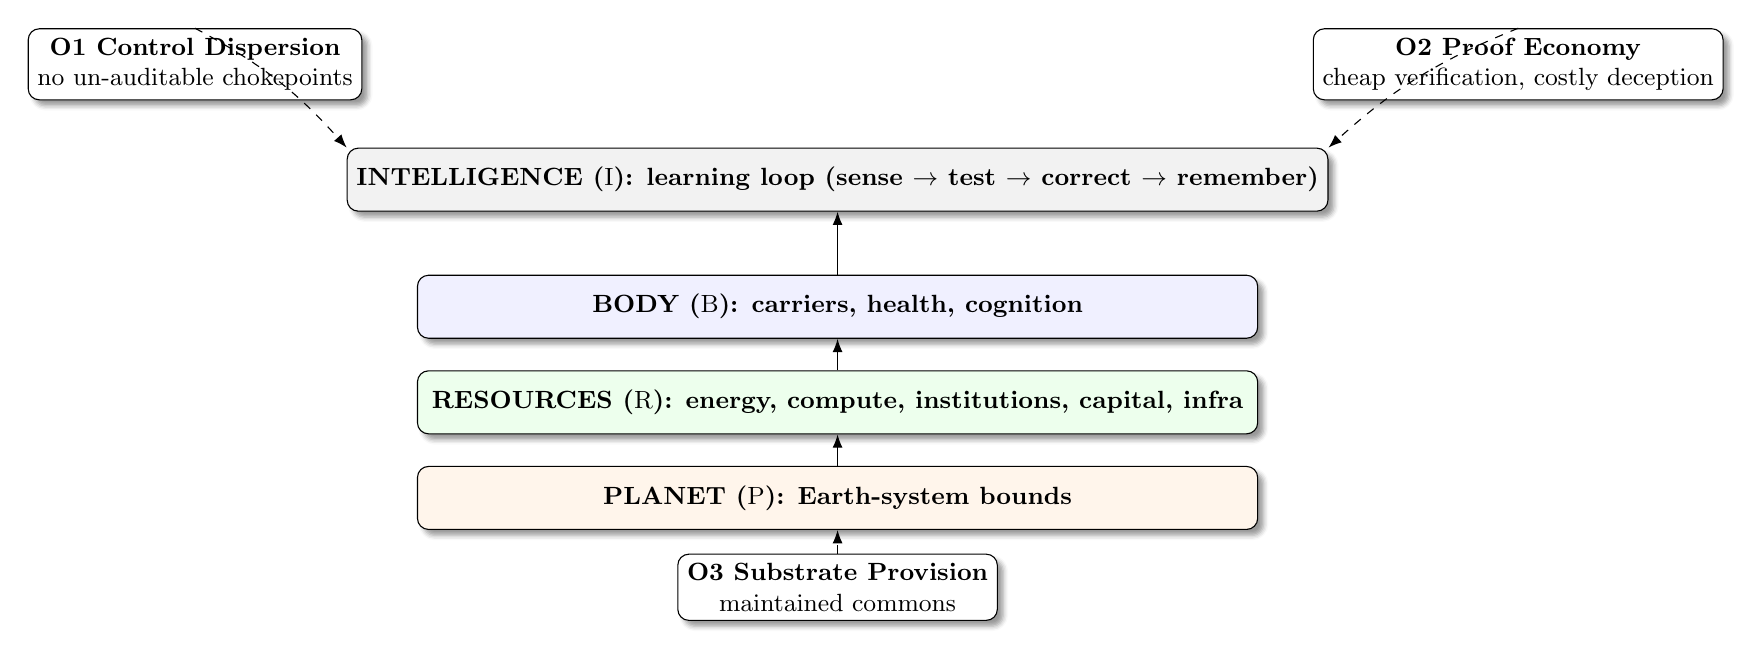
\begin{tikzpicture}[font=\small, node distance=6mm, >=Latex, every node/.style={align=center}]
  % Boxes
  \node[draw, rounded corners, fill=gray!10, minimum width=0.88\linewidth, minimum height=8mm, blur shadow] (I) {\textbf{INTELLIGENCE ($\I$): learning loop (sense $\to$ test $\to$ correct $\to$ remember)}} ;
  \node[draw, rounded corners, fill=blue!6, minimum width=0.88\linewidth, minimum height=8mm, below=8mm of I, blur shadow] (B) {\textbf{BODY ($\B$): carriers, health, cognition}};
  \node[draw, rounded corners, fill=green!7, minimum width=0.88\linewidth, minimum height=8mm, below=4mm of B, blur shadow] (R) {\textbf{RESOURCES ($\R$): energy, compute, institutions, capital, infra}};
  \node[draw, rounded corners, fill=orange!8, minimum width=0.88\linewidth, minimum height=8mm, below=4mm of R, blur shadow] (P) {\textbf{PLANET ($\Pplanet$): Earth-system bounds}};

  % Operators surrounding
  \node[draw, rounded corners, fill=white, above left=6mm and -2mm of I, blur shadow] (O1) {\textbf{O1 Control Dispersion}\\ no un-auditable chokepoints};
  \node[draw, rounded corners, fill=white, above right=6mm and -2mm of I, blur shadow] (O2) {\textbf{O2 Proof Economy}\\ cheap verification, costly deception};
  \node[draw, rounded corners, fill=white, below=3mm of P, blur shadow] (O3) {\textbf{O3 Substrate Provision}\\ maintained commons};

  % Arrows
  \draw[->] (B) -- (I);
  \draw[->] (R) -- (B);
  \draw[->] (P) -- (R);
  \draw[->, dashed] (O1.north) to[bend left=10] (I.north west);
  \draw[->, dashed] (O2.north) to[bend right=10] (I.north east);
  \draw[->, dashed] (O3.north) -- (P.south);
\end{tikzpicture}
\end{center}
\vspace{-0.5em}

For each layer, apply O1--O3. Example: at $\R$, use antitrust/interoperability (O1), machine-readable vote rationales \& open procurement (O2), and public-goods finance (O3).

\section{Alignment as Overlap of Aim and Method (OAM)}
\label{sec:oam}
\defterm{Alignment} holds when (i) agents optimise sufficiently similar aims (existence of intelligence) \emph{and} (ii) their methods do not erode others’ learning capacity or shared substrates. Helpful mechanisms: provenance, rate limits, pass-through accountability, rewarded retractions. Harmful: deception, unpriced externalities (spam, data poisoning), attention/compute monopolies, irreversibles without review.

\section{Metrics, Predictions, and Pilots}
\label{sec:metrics}

\subsection*{Minimal dashboard (public, auditable)}
\begin{itemize}[leftmargin=1.2em]
\item \textbf{Loop quality}: pilot$\to$policy ratio; replication rate; anomaly$\to$fix time; viral-correction rate.
\item \textbf{Dispersion}: HHI across attention/compute/capital/\emph{stewardship}; with-management voting rates.
\item \textbf{Substrate margins}: excess clinical capacity ($\B$); grid/compute resilience ($\R$); MRV-audited distances to planetary thresholds ($\Pplanet$).
\item \textbf{Irreversibility risk}: share of deployments with rollback plans; count of irreversibles with ex-ante review.
\end{itemize}

\subsection*{Testable predictions}
\begin{enumerate}[leftmargin=1.2em]
\item Diversity improves persistence \emph{only if} the proof economy is strong; without it, diversity degrades into noise/polarization.
\item Power concentration shortens horizon $T$ (lower replication of corrections, higher irreversibility), independent of culture.
\item Rewarding public self-correction yields super-linear gains from adding nodes; without it, systems stagnate/backslide.
\item Asset-manager/attention monopolies correlate with shrinking basins (elite impunity up, alternation of power down, local news capacity down).
\item Strengthening guardrails (antitrust/interoperability, pass-through stewardship, audit courts) predicts recovery (rollback speed up, viral corrections up).
\end{enumerate}

\subsection*{Pilots (6–12 months)}
\begin{itemize}[leftmargin=1.2em]
\item \defterm{Custodian cadence}: 3 weekly micro-habits (don’t amplify junk; buy to de-concentrate; boost watchdogs), 2 monthly group touches (show up locally; cross-tribe conversation), 1 yearly rotation (serve or substitute). Measure impacts vs matched controls.
\item \defterm{Aggregation layer}: verified petitions + sortition panels produce quarterly digests to representatives; evaluate legibility and workload.
\item \defterm{Public Goods Portfolio (PGP)}: municipal fiber + district energy + rent pool; pass-through voting; open ledgers.
\item \defterm{Learning courts sandbox}: docket for data quality, evaluation disputes, and transparency remedies.
\end{itemize}

\section{Ethics, Obstacles, and Failure Modes}
\label{sec:ethics}
\textbf{Ethical floor:} auditability, rights (due process, minority protection), corrigibility, power dispersion, proportionality, honest evidence.
\textbf{Obstacles:} capture \& concentration; Goodhart/gaming; polarization; precarity/time poverty; AI persuasion \& opacity; moral overload.
\textbf{Countermeasures:} bright-line COI rules and finance caps; metric rotation + adversarial audits + failure digests; sortition deliberation; civic slack (stipends/childcare); provenance/rate limits/liability for AI; fund public-interest media and make corrections viral.

\section{Decision Heuristic (Existence Calculus)}
\label{sec:calculus}
For any policy/tech/finance/cultural move, ask:
\begin{enumerate}[leftmargin=1.2em]
\item \textbf{Loop persistence}: does it raise the chance the learning loop keeps running (faster correction, better memory)?
\item \textbf{Boundary safety}: does it increase distance to $B^\*,R^\*,P^\*$ (or at least not reduce it)?
\item \textbf{Chokepoints}: does it disperse control (forkability, portability, pass-through), or create lock-in?
\item \textbf{Reversibility}: is rollback feasible and pre-planned?
\end{enumerate}
Proceed only if the loop’s existence probability increases and no substrate threshold is endangered.

\section{Conclusion}
\label{sec:conclusion}
We are not freezing a form; we are stabilising a \emph{learning loop}. Existence is the aim. Because the loop is substrate-dependent, maximising its persistence necessarily maintains Body, Resources, and Planet. The universal recipe is invariant across humans, AIs, and ETs: disperse control, honour proof, and provision the substrate. Democracy, markets, and AI are instruments we keep only insofar as they enlarge the basin of corrigible persistence. Freedom and diversity are not afterthoughts; they are the exploration engine inside guardrails. When rivalry and deception are governed, more nodes make intelligence rise and existence longer.

% =========================================================
\appendix
\section*{Appendix A: Ten-Line Creed}
\begin{enumerate}[leftmargin=1.2em]
\item Existence is our aim.
\item Keep the learning loop alive.
\item Disperse control---no node beyond audit or recall.
\item Honour proof---receipts, replication, retraction.
\item Sustain the substrate---body, resources, planet.
\item Protect dissent \& diversity---many bets, shared methods.
\item Choose reversibility---pilot, measure, roll back when wrong.
\item Align aim \emph{and} method---no tactics that erode others’ learning.
\item Reward the quiet custodians who keep the rules working.
\item Leave power forkable---and the future open for more minds.
\end{enumerate}

\section*{Appendix B: Custodian Contract (citizen-level)}
\textbf{Micro-habits (weekly):} do not amplify junk; buy to de-concentrate; boost a watchdog.\\
\textbf{Group touches (monthly):} show up locally; cross a tribal line.\\
\textbf{Rotation (yearly):} serve when tapped (jury/sortition) or substitute (volunteer shift or support an accountability org).\\
\textbf{Clean tactics:} no disinfo, doxxing, or intimidation; change your mind on evidence; publish receipts.\\
\textbf{Reciprocals (state):} equal enforcement; open records; anti-capture architecture; civic-skills curriculum; protected whistleblowing channels.

\section*{Appendix C: Guardrails against Capital Dominance}
\textbf{Anti-concentration:} antitrust, interoperability, data portability.\\
\textbf{Money-power firebreaks:} campaign-finance caps, lobbying transparency, COI rules.\\
\textbf{Asset-manager stewardship:} pass-through voting by default; machine-readable vote rationales; caps and periodic retenders; conflict firewalls.\\
\textbf{Public-interest media:} durable funding for investigative work and local news.

\section*{Appendix D: Public Goods Portfolio (PGP)}
\textbf{Sleeves:} (i) yielding commons (regulated utilities/infra), (ii) shared rents (land/carbon/spectrum $\to$ dividend), (iii) civic infrastructure (local news, open source, data trusts via quadratic matching).\\
\textbf{Benefits:} cash \& service dividends; pass-through voice; open ledgers.\\
\textbf{Governance:} professional fiduciaries + sortition board + technical audit committee; stewardship pluralism and open data.

\section*{Appendix E: Learning Clause (constitutional)}
\emph{Sense $\to$ Hypothesise $\to$ Test $\to$ Evaluate $\to$ Scale/Stop $\to$ Remember}.\\
Open data by default; pre-registered pilots; independent evaluation; model cards and errata; automatic sunsets and rollbacks; rights as hard stops; sortition within the loop.

\section*{Appendix F: OAM Alignment Checklist}
Aim: shared meta-objective (existence of intelligence).\\
Method: no tactics that erode others’ learning or shared substrates.\\
Resources: rivalrous resources budgeted/rationed; externalities priced.\\
Governance: audits, corrections, and rollbacks routine and low-friction.\\
Power: accumulations capped; any node removable without collapse.

% =========================================================
\section*{Acknowledgments}
This manuscript condenses a long dialogue on existence-first governance, EbE layering, capital guardrails, public-goods finance, and agent-neutral alignment.

\end{document}
